% Modified https://tex.stackexchange.com/a/484557
% https://creativecommons.org/licenses/by-sa/4.0/

\documentclass[tikz,border=2mm]{standalone}
\usetikzlibrary{shapes.geometric,calc,shapes.misc}
\begin{document}
    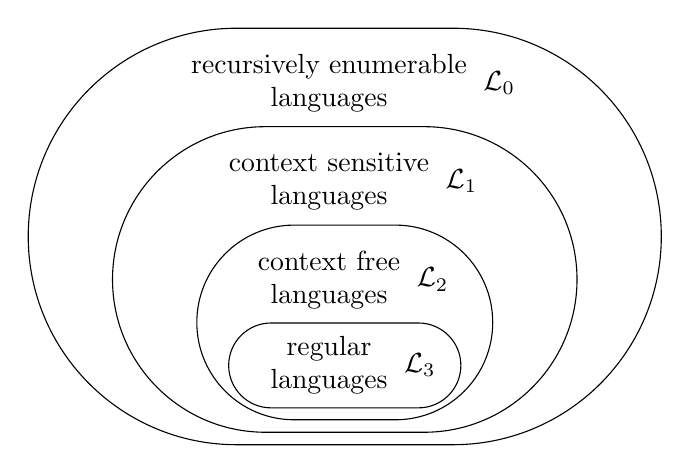
\begin{tikzpicture}[breathe dist/.initial=2ex]
    \foreach \X [count=\Y,remember=\Y as \LastY] in 
    {regular,context free,context sensitive,recursively enumerable}
     {\ifnum\Y=1
         \node[rounded rectangle,draw,outer sep=0pt] (F-\Y) {\begin{tabular}{c}\X \\ languages\end{tabular}$\mathcal{L}_3$};
     \else
      \node[anchor=south] (T-\Y) at (F-\LastY.north) {\begin{tabular}{c}\X \\ languages\end{tabular}$\mathcal{L}_{\the\numexpr4-\Y}$};
      \path let \p1=($([yshift=\pgfkeysvalueof{/tikz/breathe dist}]T-\Y.north)-(F-\LastY.south)$),
      \p2=($(F-1.east)-(F-1.west)$),\p3=($(F-1.north)-(F-1.south)$)
      in ($([yshift=\pgfkeysvalueof{/tikz/breathe dist}]T-\Y.north)!0.5!(F-\LastY.south)$) 
      node[minimum height=\y1,minimum width={\y1*\x2/\y3/1.8},
      draw,rounded rectangle,inner sep=0pt, yshift=-1ex] (F-\Y){};
     \fi}
    \end{tikzpicture}
\end{document}
